\documentclass[a4paper,12pt,titlepage]{article}
\usepackage{graphicx}
\usepackage[hidelinks]{hyperref}
\usepackage{listings}
\usepackage{float}

% Taken from Lena Herrmann at 
% http://lenaherrmann.net/2010/05/20/javascript-syntax-highlighting-in-the-latex-listings-package
\usepackage{listings}
\usepackage{color}
\definecolor{lightgray}{rgb}{.9,.9,.9}
\definecolor{darkgray}{rgb}{.4,.4,.4}
\definecolor{purple}{rgb}{0.65, 0.12, 0.82}

\lstdefinelanguage{JavaScript}{
  keywords={typeof, new, true, false, catch, function, return, null, catch, switch, var, if, in, while, do, else, case, break},
  keywordstyle=\color{blue}\bfseries,
  ndkeywords={class, export, boolean, throw, implements, import, this},
  ndkeywordstyle=\color{darkgray}\bfseries,
  identifierstyle=\color{black},
  sensitive=false,
  comment=[l]{//},
  morecomment=[s]{/*}{*/},
  commentstyle=\color{purple}\ttfamily,
  stringstyle=\color{red}\ttfamily,
  morestring=[b]',
  morestring=[b]"
}

\lstset{
   language=JavaScript,
   backgroundcolor=\color{white},
   extendedchars=true,
   basicstyle=\footnotesize\ttfamily,
   showstringspaces=false,
   showspaces=false,
   tabsize=2,
   breaklines=true,
   showtabs=false,
   captionpos=b
}

\DeclareGraphicsExtensions{.png}
\graphicspath{{./images/}}

\begin{document}
\begin{titlepage}
	\begin{center}		
		\textbf{\LARGE COS301 Mini Project \\\textbf{Testing}\\}
		\vspace{1 cm}
		\LARGE{\textbf{Notification}}
		%\begin{minipage}{0.4\textwidth}
			\begin{flushright} \large
				Johan Marx 12105202\newline
				Tim Kirker 11152402\newline
				Edwin Fullard 12048675\newline
				Matthew Russell 12047822\newline
				Jessica Lessev 13049136\newline		
				Hanrich Potgieter 12287343\newline
				Roger Tavares 10167324\newline
				Thinus Naude 13019602 \newline
				Paul Engelke 13093500\newline
			\end{flushright}
		%\end{minipage}
		\vfill
		\textbf{Git repository link:\\}
		\url{https://github.com/DianMarx/notificationTesting}
		\vfill
		{\LARGE Version}
		{\large \today}			
	\end{center}
\end{titlepage}



%-----------------TABLE OF CONTENT-----------------
\newpage
\tableofcontents
\newpage
%-----------------INTRODUCTION-----------------
\section{Introduction}

This document was compiled by our group and was produced as a whole by the team. \bigskip

We were tasked with testing the two Buzz Notification modules. The functionality provided by the buzzNotification module should be focused on a user registering to receive a notification messages.


%-----------------INTRODUCTION-----------------
\section{What we tested}
Our testing involved looking at the two notification modules and comparing it to the specification. The use cases we will be evaluated can be seen in figure ~\ref{fig:scope}
\begin{figure}[H]
	\centering
	\fbox{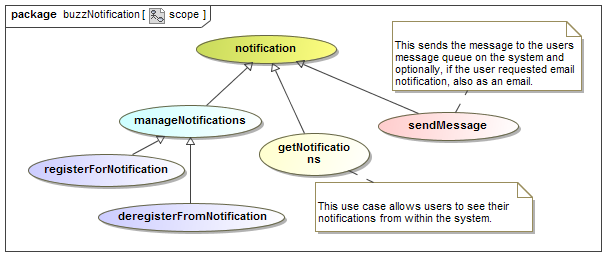
\includegraphics[width=1.0\textwidth]{scope}}
	\caption{The scope of the buzzNotification module.}
	\label{fig:scope}
\end{figure}
%-----------------PARTS-----------------
\newpage

\section{Functional Testing}
We tested each use case and made conclusion based on what we found. For all use cases of Buzz Notification A and B we will either that the use case a success or we will provide a list of violations of the contract requirements (e.g. pre- and post-condition violations or data structure requirement violations)

% Matthew
\subsection{Register for Notification Use Case}
	% Matthew Russell
We found the following problems with regards to the "Register for Notification" use case of the module.
\subsubsection*{Notification A}
The notification module for team A had the following violations
\begin{enumerate}
    \item Pre condition violations:
    \begin{itemize}
        \item Team A provided no checks for pre-conditions.
    \end{itemize}
    \item Data structure requirement violations:
    \begin{itemize}
        \item None found.
    \end{itemize}
\end{enumerate}
\subsubsection*{Notification B}
The notification module for team B had the following violations
\begin{enumerate}
    \item Pre condition violations:
    \begin{itemize}
         \item None found.
    \end{itemize}
    \item Data structure requirement violations:
    \begin{itemize}
        \item None found.
    \end{itemize}
\end{enumerate}
\subsubsection*{Remarks}
Team A provided no checks for pre-conditions  before writing data to the database, in every case the function returns with a value of true, making it appear to succeed even when there was no data written to the database at all, and thus no registration actually happened.\newline
Team B had no pre-condition violations. Any data that violated pre-conditions was correctly checked for and handled, registration of the user is only made if all the pre-conditions are successfully met.

	
% Jessica Lessev	
\subsection{Deregister for Notification Use Case}
	% Jessica Lessev
% Check template
	
% Tim Kirker	
\subsection{Send message}
	% Tim Kirker
% See template

\newpage

\section{Non-functional testing/assessment}
Problems regarding performance, scalability, maintainability, reliability, usability as well as evidence/proof of said problems.

% Johann Marx
\subsection{Performance}
	% Johann Marx
% See template
The notification module had the following problems regarding performance of the notification system both A and B. 
\subsubsection*{Notification A}
\begin{itemize}
    \item No test file.
    To start off with, Notification A had no test file to actually test the performance with.
    \item Two 
    \item Three 
    \item Four 
\end{itemize}
\subsubsection*{Notification B}
\begin{itemize}
    \item Buggy Test file
    Even though they had a test file for the coding, which was configured with nodeUnit to do unit tests etc.,
    The file did not finish the test.  It started testing, had no assertions, connected to the server, but then just stopped. This is mainly because of the .listened function which never ends automatically.
    \item Two 
    \item Three 
    \item Four 
\end{itemize}
\subsubsection*{Remarks}
Neither of the teams did what was required by the architectural requirements  ... bla bla blas write something here 
	
% Thinus Naude
\subsection{Scalability}
	% Thinus Naude
	
% Roger Tavares	
\subsection{Maintainability}
	% Roger Tavares	
% Check template 
As defined in the Architectural Requirements Document all modules should be designed and developed in such a way that they are modular allowing for sub modules to be added or even removed during development.\newline

This allows for a more maintainable system as Diagnostics of potential flaws and function clashes can now be eliminated as the system can be tested as individual parts or even as a whole allowing for a more stable module.\newline

Team A and B's modules will each be discussed below with regards to this non functional requirement:
\subsubsection*{Notification A}
\begin{itemize}
	\item The initial problem with Notification A is that all the code is part of the same Java Script file suggesting that the whole module is dependent on itself and if one function is providing the wrong functionality the whole module will fail or produce incorrect output.
	\item Opening the Java Script file one can immediately see that this module is not made of sub modules and testing is done by commenting out of code. This can produce many errors and is hard to test since you don't know which line of code is producing errors or is providing incorrect results.  
\end{itemize}

\subsubsection*{Notification B}
\begin{itemize}
	\item Notification B has sub-dived the whole notification module into smaller more manageable sub modules allowing for individual testing. 
	\item Each sub module can then be altered and tested before integrating into the final module allowing the system to be maintained at a constant stable version. New functionality can now be added via new submodules allowing for plug ability. 
\end{itemize}

\subsubsection*{Remarks}
Notification A did not meet the non functional requirement maintainability as their code is not modular while on the other hand Notification B made an excellent job to ensure that their code remains as modular as possible.

	
% Paul Engelke
\subsection{Reliability}
	% Paul Engelke (u13093500)

\subsubsection*{Notification A}
Below are some of the issues that could be identified in the module provided by Notifications A.
\begin{itemize}
    \item \textbf{Function Return Values:}\newline
     All functions available in the module's API should return some indication of success.
     However, in the case of this module, all the functions that return a value, only return true (proof of which can be found on lines 137, 169, 215, 260, 305). This means that 
     regardless of what the outcome of the function's execution is, the caller will only perceive it as 
     having succeeded --- which is an issue of reliability: if an error occurs and needs to be handled by the system, 
     nothing can be done because the function does not notify the system of erroneous execution.
     \item \textbf{Callback Usage:}\newline
     A follow-on of the previous point is the usage of callbacks.
     No provision has been made for the use of callback functions and therefore any 
     information provided by asynchronous execution cannot be conveyed to the caller. So any return value, regardless of whether it may be true or false, cannot be trusted as the asynchronous part of the function will most likely not have been completed before it returns to the caller, i.e. the return value is unreliable.\newline
     Below is a listing of the function signatures that require callbacks, but do not make provision for them:
     \begin{lstlisting}
     line 94  : notification.notifyRegistration(jsonObject)
     line 140 : notification.notifyDeregistration(jsonObject)
     line 172 : notification.notifyNewPost(jsonObject)
     line 218 : notification.notifyDeletedThread(jsonObject)
     line 263 : notification.notifyMovedThread(jsonObject)
     line 308 : notification.appraisalRegister(jsonObject)
     line 321 : notification.appraisalDeregister(jsonObject)
     line 336 : notification.appraisalNotify(jsonObject)
     line 390 : notification.sendNotification(jsonObject)
     \end{lstlisting}
     \item \textbf{Logging to Console:}\newline
     In the cases where errors occur and in some cases where successful execution occurs, information about the success or failure is lost to the system as it is only logged to the console(not reliable as a persistence tool) instead of being returned in some form that the caller can interpret. This is another issue of reliability as the system cannot determine whether or not a user will now receive notifications or if a user has been deregistered from receiving notifications, etc.
\end{itemize}
\subsubsection*{Notification B}
\begin{itemize}
	\item Issue 1
\end{itemize}
\subsubsection*{Remarks}
[Remarks go here...]

% Hanrich Potgieter		
\subsection{Integrability}
	% Hanrich Potgieter		
% Check 
subsubsection*{Integratability A}
We tested the Integratability of the following fucntions. These functions has been supplied by group A
\begin{itemize}
	\item Installing required Packages
	There is no way of installing the required packages.
	\item Dependancy Injection
	There is no dependacy injection.
	\item Unit tests
	There was no supplied unit test. Therefore we cannot test if the functions is working.
\end{itemize}
\subsubsection*{Integratability B}
The integratability of notification B is not adequite. There are numerbour challanges that are missing. There is no dependancy injection and all packages needs to be installed manually.
\begin{itemize}
	\item File Structure 
	Each function is placed in a seperate file. There is no common module to integrate that will allow access to all the capabilities of notifications.
	\item Installing required packages
	One cannot easily install the dependancys that is required by Notifications.
	\item Dependancy Injection
	There is no dependacy injection.
	\item Unit tests
	There was no supplied unit test. Therefore we cannot test if the functions is working. There is a file called allTogether.js that is an attempt at unit testing but no proper unit testing was applied.
	\item Four 
\end{itemize}
\subsubsection*{Remarks}
Notification B is not Integratable at alll. There is no provision for dependacny injection.
	
% Trevor Austin
\subsection{Usability}
	% Trevor Austin (u11310856)
The issues related to usability and the testing of usability are included below:
\subsubsection{Notification A Usability Testing}
\begin{itemize}
	\item The first and foremost problem is there is no way to test if the notification section is usable as no testing infrastructure for usability is provided. The team would need to implement just a basic interface to allow users to actually use the functions they have implemented. Thus, without this in place the notification module has no real usability. In order to provide a full usability testing section, the authors have assumed that there is a functioning interface for some of the points below.
	\item There was no testing interface that functioned correctly. This prevented further usability tests as the tester could not see if the functions were procedurally correct. All 18 of the 18 tests failed when attempting to use nodeunit(the testing infrastructure that was provided). This can be seen in the figure \ref{fig:usabFailA}. This shows further that the module, even with a functioning interface, would not be able to have any usability.
	\begin{figure}[h!]
		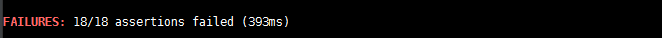
\includegraphics[width=\linewidth]{../images/Failure.png}
		\caption{Usability test failure}
		\label{fig:usabFailA}
	\end{figure}
	\item The call-back nature of many of the functions, as mentioned in previous sections, is lacking. Many of the functions that are called return Boolean values but they do not use call-back functions in order to return these functions. This in combination with the asynchronous nature of JavaScript, or node.js, causes the values to always return true values. With relation to usability, the user would always assume that when they register for a notification, unregister, or even opt in for e-mail notifications. This proves to be false as the functions do not return properly which can cause frustration for the user as the program does alter values as expected. The usability for the function calls within the module is null.
	\item Similar to the above point, none of the functions throw errors. This prevents notification to user of problems within the application. The user would become frustrated as they would not be able to understand why the program is not functioning correctly. The user would not be able to provide specific debugging information as feedback to the developers.
	\item NPM install of the module does not function at all(See Figure \ref{fig:npmFailA} below) . So with regards to usability for developers the module has failed.
	\begin{figure}[h!]
		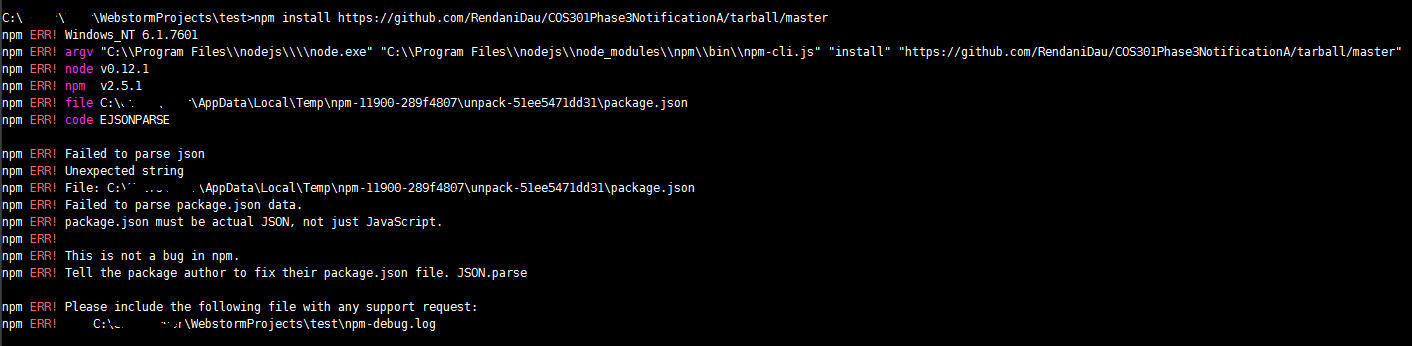
\includegraphics[width=\linewidth]{../images/npmfail.png}
		\caption{NPM Failure}
		\label{fig:npmFailA}
	\end{figure}
	\item The programs code is poorly commented but at least maintains some concept of simplicity.
\end{itemize}
\subsubsection{Notification B Usability Testing}
\begin{itemize}
	\item The usability for developers is lacking. The npm install of the module does not give all the required files for testing to work. The tester had to manually install some of the modules as they required to see if the testing program runs. Usability on a developer level is substandard. 
	\begin{figure}[h!]
		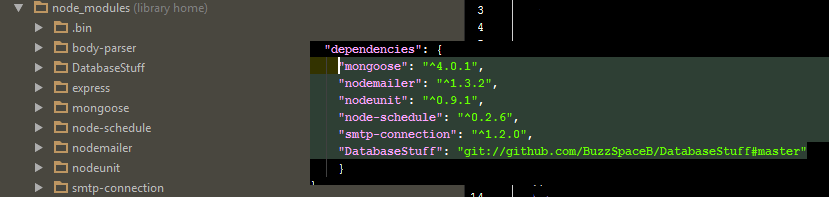
\includegraphics[width=\linewidth]{../images/Dependencies.png}
		\caption{Dependency Failure}
		\label{fig:depFailA}
	\end{figure}
	\item Notification B did provide a testing file which seems to emulate the idea of sending e-mail notifications. The problem with this system is that many of the functions fail to execute. This can cause frustration for the users as the they would not receive expected notifications from services. Thus the required usability is not met.
	\begin{figure}[h!]
		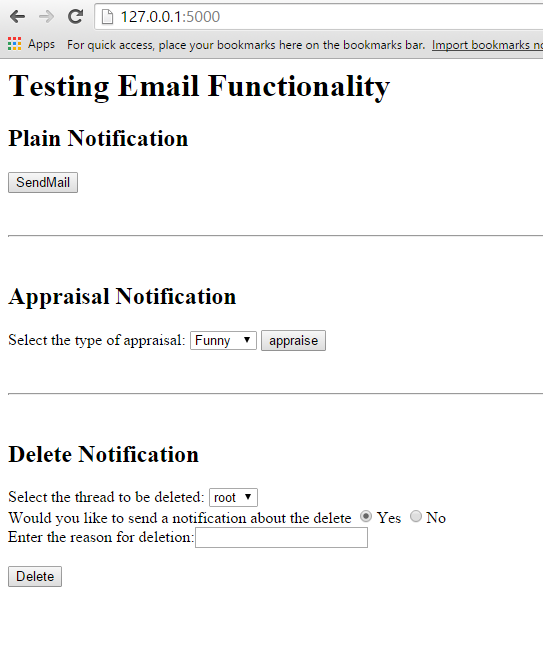
\includegraphics[width=\linewidth]{../images/Interface.png}
		\caption{Emulated Interface}
		\label{fig:emuInterface}
	\end{figure}
	\item In aspects of programmer usability, the code is poorly commented in some sections and near perfect in others. The code is poorly structured and creates an overall impression of disorganisation
	\item Similar to above with regards to callbacks and thrown errors. The difference being that some errors are thrown. 
\end{itemize}
\subsubsection{Remarks}
The overall impression of both notication sections is that they did not meet the requirements that were needed. The usability was substandard and a lot of improvement is needing for a fully deployable product.

	

\end{document}
